\documentclass[a4paper]{leaflet}

% \usepackage[utf-8]{inputenc}
\usepackage[right]{eurosym}
\usepackage{longtable}
\usepackage{graphics}
\usepackage[ngerman,frenchb]{babel}

% \usepackage[tmargin=1in,bmargin=1in,lmargin=1.25in,rmargin=1.25in]{geometry}

\usepackage{xcolor}
\usepackage{titlesec}

\definecolor{MSBlue}{rgb}{.204,.353,.541}
\definecolor{MSLightBlue}{rgb}{.31,.506,.741}

% Set formats for each heading level
\titleformat*{\section}{\Large\bfseries\sffamily\color{MSBlue}}
\titleformat*{\subsection}{\large\bfseries\sffamily\color{MSLightBlue}}
\titleformat*{\subsubsection}{\itshape\subsubsectionfont}


\setmargins{12mm}{12mm}{12mm}{12mm} %oben, unten, links, rechts


% Finally, give us PDF bookmarks
\usepackage{color,hyperref}
\definecolor{darkblue}{rgb}{0.0,0.0,0.3}
\hypersetup{colorlinks,breaklinks,
	linkcolor=darkblue,urlcolor=darkblue,
	anchorcolor=darkblue,citecolor=darkblue}



\begin{document}

\sffamily

% \fboxsep2mm
% \fbox{
    \begin{minipage}{8.2cm}

		\begin{center}
	
		\vspace{42pt}
	
		
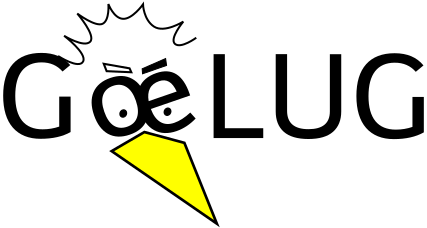
\includegraphics[width=5.5cm]{../logo/goelug_proposition1/goelug_logo_t1}
% 
\includegraphics[width=2.5cm]{goeland}

Linux User Group --- Le Havre

\vspace{18pt}

\huge

Go\'{e}LUG

%\vspace{32pt}

\normalsize

\href{http://www.goelug.org}{\tt www.goelug.org}

\vspace{18pt}

Association de promotion et de d\'{e}fense du logiciel libre

\vspace{42pt}

\textsf{Nos permanences:} \\[11pt]
$ 1^{er} $ Jeudi du mois $ 18^{00} $ - $ 21^{00} $ \\

\vspace{34pt}

A la cantine numerique du Havre \\
Le Container \\
\href{http://www.lecontainer.co}{\tt www.lecontainer.co}


		\vspace{52pt}
		
		\end{center}

    \end{minipage}
% }

\newpage



\section*{Linux User Group}

\dots

\subsection*{L'association}

\dots

\subsection*{GNU et les logicielles libre}

\dots

\section*{Evenements} 

Notre perimetre d'action

\subsection*{D'ecouverte de systemes GNU/Linux}


\subsection*{Install Parties}

La distribution pour vos besoins.

\subsection*{Goebiduille}

\begin{itemize}
\item RPI,
\item Arduino
\end{itemize}

\href{http://www.recalbox.com/}{\tt http://www.recalbox.com/}

\subsection*{Conferences}


\href{http://www.linuxfoundation.org/}{\tt http://www.linuxfoundation.org/}




\begin{center}
\textsf{
	Pour plus d'informations: \\
	\href{mailto:contact@goelug.org}{\tt contact@goelug.org}
}

\href{http://www.goelug.org}{\tt www.goelug.org}
	
\end{center}

\end{document}
